\documentclass[10pt]{article}
\usepackage[T1]{fontenc}
\usepackage{mathptmx}
\usepackage[margin=1in]{geometry}
\usepackage{booktabs}
\usepackage{graphicx}
\usepackage{amsmath}
\usepackage{caption}
\usepackage[colorlinks=true,urlcolor=blue,linkcolor=blue,citecolor=blue]{hyperref}
\usepackage{xurl}
\captionsetup{font=small,labelfont=bf,skip=4pt}
\setlength{\parskip}{3pt}
\setlength{\parindent}{0pt}
\graphicspath{{../results/}}
\newcommand{\usi}{\textit{URLSimilarityIndex}}

\title{Replicating and Critiquing PhiUSIIL Phishing URL Detection\\Under Dataset Shift}
\author{Suyash Pradeep Muley\\Replication and Critique project, Northeastern University\\{\small Draft 1, \today}}
\date{}

\begin{document}
\maketitle

\begin{abstract}
\noindent
Prasad and Chandra (2024) report 99.24\% accuracy for an incremental phishing URL detector on the PhiUSIIL dataset. I reproduce their Tables 3, 5, 6 and 7 to within about 0.001 accuracy, and then ask two questions the paper does not: what does that number depend on, and does a URL-only detector keep its operating point on independent sources? The headline does not depend on the similarity index: removing it changes BestSecurity accuracy by 0.0001, and URL-only features alone still reach 0.987. The index is a construction shortcut (legitimate URLs come from the list it is matched against), not label leakage. In a transfer study with matched pool size and class mix, registered-domain-disjoint splits, and thresholds fixed at 95\% recall on source validation data, models trained on PhiUSIIL, GramBeddings or PhreshPhish do not carry their operating point to the other sources: recall on a target ranges from 0.52 to 0.98 and false-positive rate from 0.00 to 1.00 (HistGB), in opposite directions for different source pairs. The sources are separable from the URL alone within each class, and normalizing URL formatting does not repair transfer. These differences look like properties of how the sources were assembled, so a larger sample from the same sources is unlikely to remove them.
\end{abstract}

\section{Introduction}
A detector that scores 99\% on one benchmark says little about how it behaves on URLs from another source. Phishing URL benchmarks are assembled by combining a feed of phishing URLs with a separate list or crawl of legitimate URLs, so the two classes can differ in ways unrelated to phishing: how URLs are written, which sites are listed, when they were collected. This report examines one widely used benchmark, PhiUSIIL \cite{prasad2024}, with two questions.

\textbf{Q1: What does the headline result depend on?} I reproduce the paper's protocol and test whether its main feature, a similarity index computed against a list of popular sites, is a source of label leakage or a dataset shortcut, and whether the result survives its removal.

\textbf{Q2: Does a URL-only detector keep its operating point on other sources?} I train on one source, fix the decision threshold using only that source's validation data, and measure recall and false-positive rate on the others, with pool size and class mix matched across sources.

Contributions:
(1) a reproduction of Tables 3, 5, 6 and 7 of the paper, with row-order variation and feature-group ablations (Section~\ref{sec:parta});
(2) a precise statement of why the similarity index is a construction shortcut and not label leakage, with evidence that URL form and page content separate the classes redundantly (Section~\ref{sec:shortcut});
(3) a transfer study over three sources, PhiUSIIL, GramBeddings and PhreshPhish, with a fourth phishing-only check, using validation-fixed thresholds (Section~\ref{sec:partb});
(4) direct measurements of how the sources differ and a test showing that normalizing URL form does not fix transfer (Section~\ref{sec:why}).

\section{Background and related work}
\textbf{PhiUSIIL.} Prasad and Chandra \cite{prasad2024} build a dataset of 235,795 URLs (134,850 legitimate, 100,945 phishing) with page-content features, and a two-phase detector. Phase 1 computes a character-match similarity index (USI, 0--100) between a URL and a list of the top 10 million sites from Open PageRank; a score of 100 is classed legitimate, 80--99 phishing. Phase 2 feeds remaining URLs to three incremental learners (BernoulliNB, PassiveAggressive, SGD) evaluated prequentially (predict a record, then \texttt{partial\_fit} on it) and combined by voting into LowSecurity, BestSecurity and HighSecurity profiles. The paper reports no test on data from another source.

\textbf{Related work.} I could not read the full text of the Elsevier and IEEE papers below, so their numbers are quoted at the level I verified (abstract unless stated). Ahamed et al.\ \cite{ahamed2026} evaluate LR, XGBoost, CharCNN and BERT on PhiUSIIL and report clean test accuracy of 0.996--0.998, falling to 0.73--0.87 on a dual-source external test, with false-positive rates of 0.25--0.54 on benign sites from a popularity list. Misiek and Hyla \cite{misiek2026} validate XGBoost across three datasets, including GramBeddings and PhiUSIIL, and report 77.8\% average accuracy on the three test sets. Rashid et al.\ \cite{rashid2024} show that unsupervised domain adaptation improves cross-dataset F1 by about 0.06 on average. Rahman et al.\ \cite{rahman2026}, whose full text I read, show that two PhiUSIIL features (the similarity index and a social-network flag) reach 99.63\% accuracy and a single AND rule 99.67\%, which agrees with the shortcut I find in Section~\ref{sec:shortcut}. Arp et al.\ \cite{arp2022} catalogue pitfalls in security machine learning, including sampling bias and spurious correlations; the present study is a concrete case of both.

\textbf{What is different here.} The cross-dataset studies above report accuracy, F1 or false-positive rate; from the abstracts alone I cannot tell whether the threshold, pool size, class mix and URL type were controlled across sources. Here I fix and report all of them explicitly: the threshold on source validation data only, matched pool size and class mix, no shared domains, and URL-type slices. I also measure directly how the sources differ, and add PhreshPhish \cite{dalton2025}, a later, independently collected dataset, as a third source. None of these papers, nor GramBeddings, appears in the PhiUSIIL paper's reference list (I searched the text of the PDF); the paper was accepted on 16 October 2023, before all of them.

\textbf{Claims of the paper that this study can test.} Three statements in the paper's discussion (its Section 5.7) bear on the questions above. First, it concludes that PhiUSIIL ``outperforms the existing state-of-the-art models'' from its Table 8, which sets its accuracy (0.9924 and 0.9979) beside ten earlier studies, each measured on its own dataset of 3,000 to 100,000 URLs; accuracy on different datasets is not a like-for-like comparison. Second, it states that the constructed dataset ``enhances model generalization'', but reports no test on data from another source, which Part B supplies. Third, it says its Table 7 shows ``a direct correlation between the dataset size and the model's performance''; in my reproduction this holds for the sequential split but not for the random split (Section~\ref{sec:parta}). Also, the paper's own batch baselines (its Table 3, for example random forest at 0.99982) score above its incremental ensemble (0.99239), so the framework's case rests on adaptability, not accuracy.

\section{Data}
\begin{table}[t]
\centering\footnotesize
\caption{Sources. ``Used'' is what the experiments read. Provenance is as documented by each source; ``not stated'' means I found no statement.}
\label{tab:data}
\begin{tabular}{p{0.8in}p{1.05in}p{1.2in}p{2.65in}}
\toprule
\textbf{Source} & \textbf{Size} & \textbf{Collected} & \textbf{Provenance as documented}\\
\midrule
PhiUSIIL & 235,795 (134,850 legitimate, 100,945 phishing); Part B uses the 235,370 unique URLs & phishing 2022-10-01 to 2023-05-21 & Legitimate: Open PageRank top-10M list. Phishing: PhishTank, OpenPhish, MalwareWorld \cite{prasad2024}.\\
GramBeddings & 800,000 (400,000 each); Part B uses a 100,000-row balanced sample & May 2019 to June 2021, one session per week & Legitimate: authors' crawler with a manual filter of near-identical domains. Phishing source, crawler seeds and verification: not stated \cite{gram}.\\
PhreshPhish & 666,315 (298,326 phishing, 367,989 benign); Part B uses a 100,000-row balanced sample & dates in the data: 2024-07-02 to 2025-12-16 & Described in \cite{dalton2025}; I make no claim about its collection beyond the measurements below.\\
PhishTank snapshot & 76,451 phishing only & snapshot of 2026-10-01 & Online-valid feed file. No legitimate class, so only recall is meaningful.\\
\bottomrule
\end{tabular}
\end{table}

Table~\ref{tab:data} lists the sources. Part A uses PhiUSIIL as released, in file order. Part B uses 22 URL-only lexical features extracted by one function for every source (Section~\ref{sec:partb}), and never the similarity index or page content. The URL form differs strongly by source and class (Table~\ref{tab:profile}). All PhiUSIIL legitimate URLs are bare \texttt{https://www.} homepages and none ends in ``/'', while 93\% of PhreshPhish and 85\% of GramBeddings legitimate URLs are deep links. Even among homepage URLs, the share ending in ``/'' ranges from 0.00 to 1.00 across sources for the legitimate class.

\begin{table}[t]
\centering
\caption{URL form by source and class. Shares of rows. ``hp'' columns restrict to homepage URLs (nothing after the host); ``Homepage share'' and ``https (all)'' use all rows of the class.}
\label{tab:profile}
{\footnotesize\setlength{\tabcolsep}{4pt}
\begin{tabular}{llrrrrrr}
\toprule
\textbf{Source} & \textbf{Class} & \textbf{Rows} & \textbf{Homepage share} & \textbf{Trailing / (hp)} & \textbf{www (hp)} & \textbf{https (hp)} & \textbf{https (all)} \\
\midrule
PhiUSIIL & legitimate & 134{,}850 & 1.00 & 0.00 & 1.00 & 1.00 & 1.00 \\
 & phishing & 100{,}520 & 0.72 & 0.44 & 0.54 & 0.39 & 0.49 \\
GramBeddings & legitimate & 50{,}000 & 0.15 & 0.53 & 0.39 & 0.49 & 0.59 \\
 & phishing & 50{,}000 & 0.12 & 0.99 & 0.10 & 0.45 & 0.47 \\
PhreshPhish & legitimate & 50{,}000 & 0.07 & 1.00 & 0.52 & 0.98 & 0.98 \\
 & phishing & 50{,}000 & 0.45 & 0.66 & 0.07 & 0.83 & 0.86 \\
PhishTank & phishing & 76{,}448 & 0.37 & 0.81 & 0.03 & 0.82 & 0.91 \\
\bottomrule
\end{tabular}
}

\end{table}

\section{Part A: reproduction of the paper}\label{sec:parta}
\textbf{Protocol.} I follow the paper: initialize on the first record, then for every later record predict and then \texttt{partial\_fit}; BernoulliNB, PassiveAggressive and SGD with the published hyperparameters; three voting profiles with legitimate as the positive class; feature selection by tree-model importance followed by the top 85\% by mutual information (43 of 50 candidate features kept; the paper does not state its final count). The paper's row order is not stated, so I report the file order and four shuffled orders (mean and sample standard deviation). Deviations: LightGBM and XGBoost were not installed, so scikit-learn models stand in for importance ranking and for the boosting rows of Table 3; mutual information was computed on a 30,000-row subsample; no feature scaling for the incremental learners.

\textbf{Results.} Tables~\ref{tab:t5} and~\ref{tab:t6} compare with the paper. BestSecurity accuracy is 0.9934 in file order and 0.9915 (sd 0.0002) over shuffled orders, against 0.9924 published; the rankings of the three profiles match. LowSecurity varies with row order (sd 0.012) because it depends on how quickly the least confident learner catches up. Confusion counts differ by a few hundred rows in the error cells. For example, BestSecurity false positives are 1,208 in file order and 1,564 on average when shuffled, against 1,539 published, and false negatives are higher than published (447 against 256). I did not investigate why. The pre-training experiment (Table 7 of the paper, Table~\ref{tab:t7} here) is reproduced to a mean absolute gap of 0.0004 (sequential split) and 0.0005 (random split); the paper does not say which split it used. The paper states that its Table 7 shows a direct correlation between dataset size and accuracy; here accuracy rises with the pre-training share in the sequential split (0.9955 at 10\% to 0.9984 at 90\%) but is flat from 60\% on in the random split (0.9980--0.9981). The batch baselines (Table~\ref{tab:t3} in the appendix) agree for the incremental-type models (BernoulliNB 0.988 against 0.986) and are near 1.000 for the tree ensembles on the selected features.

\begin{table}[t]
\centering
\caption{Reproduction of the paper's Table 5 (accuracy, F1, MCC). Legitimate is the positive class. Mean (sd) over four shuffled row orders.}
\label{tab:t5}
{\footnotesize
\begin{tabular}{llrrr}
\toprule
\textbf{Profile} & \textbf{Metric} & \textbf{Ours, file order} & \textbf{Ours, shuffled (4 runs)} & \textbf{Paper} \\
\midrule
LowSecurity & accuracy & 0.8944 & 0.8978 (0.0118) & 0.8826 \\
 & F1 & 0.9155 & 0.9180 (0.0086) & 0.9069 \\
 & MCC & 0.7974 & 0.8037 (0.0215) & 0.7760 \\
\addlinespace
BestSecurity & accuracy & 0.9934 & 0.9915 (0.0002) & 0.9924 \\
 & F1 & 0.9942 & 0.9926 (0.0002) & 0.9934 \\
 & MCC & 0.9864 & 0.9826 (0.0005) & 0.9845 \\
\addlinespace
HighSecurity & accuracy & 0.9730 & 0.9716 (0.0006) & 0.9741 \\
 & F1 & 0.9758 & 0.9746 (0.0006) & 0.9768 \\
 & MCC & 0.9467 & 0.9441 (0.0012) & 0.9488 \\
\bottomrule
\end{tabular}
}

\end{table}
\begin{table}[t]
\centering
\caption{Reproduction of the paper's Table 6, file order: confusion counts, ours / paper.}
\label{tab:t6}
{\footnotesize
\begin{tabular}{lrrrr}
\toprule
\textbf{Profile} & \textbf{TP (ours / paper)} & \textbf{TN} & \textbf{FP} & \textbf{FN} \\
\midrule
LowSecurity & 134846 / 134849 & 76046 / 73259 & 24899 / 27686 & 3 / 1 \\
BestSecurity & 134489 / 134594 & 99737 / 99406 & 1208 / 1539 & 360 / 256 \\
HighSecurity & 128490 / 128768 & 100937 / 100918 & 8 / 27 & 6359 / 6082 \\
\bottomrule
\end{tabular}
}

\end{table}
\begin{table}[t]
\centering
\caption{Pre-training experiment (the paper's Table 7): BestSecurity accuracy on the incremental part after pre-training on the first $p$\%.}
\label{tab:t7}
{\footnotesize
\begin{tabular}{lrrr}
\toprule
\textbf{Pre-train} & \textbf{Paper} & \textbf{Ours, sequential} & \textbf{Ours, random} \\
\midrule
10\% & 0.99573 & 0.99545 & 0.99622 \\
20\% & 0.99593 & 0.99630 & 0.99709 \\
30\% & 0.99637 & 0.99741 & 0.99747 \\
40\% & 0.99708 & 0.99712 & 0.99721 \\
50\% & 0.99725 & 0.99747 & 0.99759 \\
60\% & 0.99751 & 0.99799 & 0.99799 \\
70\% & 0.99755 & 0.99785 & 0.99808 \\
80\% & 0.99763 & 0.99813 & 0.99796 \\
90\% & 0.99792 & 0.99839 & 0.99796 \\
\bottomrule
\end{tabular}
}

\end{table}

\textbf{What the headline depends on.} I re-ran the full pipeline, including feature selection, with feature groups removed (Table~\ref{tab:ablation}). Removing the similarity index changes BestSecurity accuracy by 0.0001. Removing page-content features while keeping the index lowers it to 0.9726, and removing both gives 0.9870 using only URL-derived columns. So the 99\% result is reproducible from URL form alone and is not evidence that the model generalizes. (Removing page content while keeping the index is worse than removing both; I did not investigate this.)

\begin{table}[t]
\centering
\caption{BestSecurity under the paper's protocol with feature groups removed (selection re-run each time). Shuffled: mean (sd) over four orders.}
\label{tab:ablation}
{\footnotesize
\begin{tabular}{lrrrrr}
\toprule
\textbf{Features} & \textbf{Features kept} & \textbf{Accuracy, file order} & \textbf{Accuracy, shuffled} & \textbf{F1, shuffled} & \textbf{FP / FN (shuffled mean)} \\
\midrule
all & 43 & 0.9934 & 0.9915 (0.0002) & 0.9926 (0.0002) & 1564 / 447 \\
drop USI & 42 & 0.9932 & 0.9914 (0.0001) & 0.9925 (0.0001) & 1671 / 364 \\
drop page content & 19 & 0.9717 & 0.9726 (0.0004) & 0.9760 (0.0003) & 3408 / 3062 \\
drop USI and page content & 18 & 0.9879 & 0.9870 (0.0005) & 0.9887 (0.0004) & 2046 / 1014 \\
\bottomrule
\end{tabular}
}

\end{table}

\section{Shortcut check on the similarity index}\label{sec:shortcut}
The index uses no labels: the paper defines it as a character-match score against the Open PageRank list. The legitimate class was drawn from that same list, so every legitimate URL matches itself and scores exactly 100 by construction; I confirm this for all 134,850 legitimate URLs. Phishing URLs score 100 for 786, 80--99 for 7,341 (the paper's Section 5.4 reports the same 7,341), and below 80 for 92,818. The rule ``USI $<$ 100 $\Rightarrow$ phishing'' reaches accuracy 0.9967 with no legitimate URL flagged. I therefore call the index a \emph{construction shortcut}: membership in the list that generated one class. It is not label leakage, because it is computed from the URL alone.

The index is also redundant (Table~\ref{tab:shortcut}). Without it, HistGB still separates the classes (AUROC 1.0000), and a domain-disjoint split changes nothing, so this is not domain memorization. Two other artifacts separate the classes: URL form (all legitimate URLs are \texttt{https://www.}\,homepages; a rule on that form alone reaches accuracy 0.9956 with no legitimate URL flagged) and page content (83.4\% of phishing pages have zero images against 1.0\% of legitimate pages; median line count 12 against 1,105).

What I do not show: the Tranco list is a proxy I could check, but only 33.1\% of legitimate registered domains appear in its top million, as expected for a 1M list against a 10M list, so ``all legitimate URLs are in the Open PageRank list'' rests on the paper's text. I did not test why many phishing pages are empty captures. For legitimate URLs the index and the \texttt{www}-homepage form are perfectly confounded, so I cannot say which one a model uses.

\begin{table}[t]
\centering
\caption{Feature-group ablation with HistGB, mean of three seeds: AUROC / accuracy.}
\label{tab:shortcut}
{\footnotesize
\begin{tabular}{lrrr}
\toprule
\textbf{Feature set} & \textbf{n} & \textbf{Random split (AUROC / accuracy)} & \textbf{Domain-disjoint split} \\
\midrule
all features & 50 & 1.0000 / 1.0000 & 1.0000 / 1.0000 \\
without USI & 49 & 1.0000 / 0.9999 & 1.0000 / 1.0000 \\
without page content (keeps USI) & 22 & 0.9999 / 0.9998 & 0.9998 / 0.9998 \\
page content only & 28 & 1.0000 / 0.9984 & 0.9999 / 0.9977 \\
without USI and page content & 21 & 0.9988 / 0.9971 & 0.9990 / 0.9971 \\
URL columns only & 18 & 0.9985 / 0.9976 & 0.9986 / 0.9979 \\
USI only & 1 & 0.9946 / 0.9954 & 0.9927 / 0.9940 \\
\bottomrule
\end{tabular}
}

\end{table}

\section{Part B: URL-only transfer}\label{sec:partb}
\textbf{Design.} Part B is separate from the reproduction and uses only 22 URL-only features (lengths, counts of dots, hyphens, digits and special characters, path depth, number of subdomains, https and \texttt{www} flags, IP host, port, entropy, count of suspicious tokens). Every source variant is sampled to the same pool of 11,666 rows at a 50\% phishing share; this size is set by the smallest variant, the homepage-only GramBeddings sample. Each pool is split 70/15/15 so that no registered domain (eTLD+1) appears in more than one part; because domain groups differ in size, the training sets then have 7,728 to 8,566 rows, and Table~\ref{tab:mix} in the appendix lists the class and URL-type mix of every set. The decision threshold is the score at which 95\% of \emph{source validation} phishing is detected, and it is applied unchanged to every target. Target rows whose URL or registered domain appears in the training data are removed. Targets are the source's own test split, each other dataset (all rows, homepage-only, deep-only), and PhishTank (phishing only). Models: logistic regression, random forest (200 trees), HistGB (300 iterations), an MLP (64, 32), and logistic regression on character 2--4-gram TF-IDF of the URL string. I run three feature sets (all; without the https flag; without the https and \texttt{www} flags) and five seeds. PhiUSIIL has no deep-link legitimate URLs, so its training set cannot be balanced by URL type; I instead evaluate every target by URL type.

\textbf{Main result.} Table~\ref{tab:main} and Figure~\ref{fig:op} show the operating point at the fixed threshold. In-source, the threshold works: recall is 0.93--0.98 for all five models. On other sources it does not, and the failure differs by direction.
\begin{itemize}
\item Trained on PhiUSIIL, HistGB flags almost everything on GramBeddings (FPR 0.81) and PhreshPhish (FPR 0.73) while keeping recall (0.98, 0.88).
\item Trained on GramBeddings, it misses about half of PhiUSIIL phishing (recall 0.53) at FPR 0.00, and on PhreshPhish reaches recall 0.77 at FPR 0.28.
\item Trained on PhreshPhish, it flags every PhiUSIIL URL (FPR 1.00, AUROC 0.49, no better than chance) and has FPR 0.68 on GramBeddings.
\end{itemize}
The oracle FPR column shows that a threshold tuned on the target would not rescue most pairs: for HistGB the FPR at 95\% recall is 0.70--1.00 on every cross-source pair, so the ranking itself, not only the threshold, fails to transfer. The pattern in recall and FPR agrees across the five models (Figure~\ref{fig:op}). Pair-level AUROC does not: for PhreshPhish $\to$ PhiUSIIL it ranges from 0.27 (random forest) to 0.99 (character n-grams), and the 0.99 is an artifact of the scheme and \texttt{www} text (it falls to 0.72 without them, Section~\ref{sec:why}). I therefore lead with recall and FPR at the fixed threshold and treat pair-level AUROC as model dependent. PR-AUC is in Table~\ref{tab:prauc} in the appendix; it depends on the phishing share of each target, which differs between targets, so I do not compare it across them.

\begin{table}[t]
\centering
\caption{Transfer at the validation-fixed threshold (95\% recall on source validation). HistGB, mean$\pm$sd over five seeds. Oracle FPR: FPR at 95\% recall if the threshold were chosen on the target (diagnostic only). Last two columns: range of the mean over the five models.}
\label{tab:main}
{\scriptsize\setlength{\tabcolsep}{3.5pt}
\begin{tabular}{llrrrrrr}
\toprule
\textbf{Trained on} & \textbf{Tested on} & \textbf{AUROC} & \textbf{Recall} & \textbf{FPR} & \textbf{Oracle FPR} & \textbf{Recall, 5 models} & \textbf{FPR, 5 models} \\
\midrule
PhiUSIIL & in-source test & 1.00$\pm$0.00 & 0.93$\pm$0.03 & 0.00$\pm$0.00 & 0.00 & 0.93-0.94 & 0.00-0.00 \\
 & GramBeddings & 0.76$\pm$0.03 & 0.98$\pm$0.01 & 0.81$\pm$0.05 & 0.72 & 0.95-0.99 & 0.66-0.95 \\
 & PhreshPhish & 0.67$\pm$0.04 & 0.88$\pm$0.03 & 0.73$\pm$0.13 & 0.96 & 0.80-0.89 & 0.40-0.97 \\
\addlinespace
GramBeddings & in-source test & 0.94$\pm$0.01 & 0.94$\pm$0.01 & 0.29$\pm$0.04 & 0.32 & 0.93-0.95 & 0.15-0.47 \\
 & PhiUSIIL & 0.83$\pm$0.02 & 0.53$\pm$0.04 & 0.00$\pm$0.00 & 0.84 & 0.50-0.58 & 0.00-0.02 \\
 & PhreshPhish & 0.80$\pm$0.01 & 0.77$\pm$0.03 & 0.28$\pm$0.03 & 0.70 & 0.68-0.82 & 0.18-0.39 \\
\addlinespace
GramBeddings (homepage only) & in-source test & 0.95$\pm$0.02 & 0.96$\pm$0.01 & 0.30$\pm$0.04 & 0.26 & 0.95-0.97 & 0.21-0.33 \\
 & PhiUSIIL & 0.82$\pm$0.02 & 0.52$\pm$0.03 & 0.00$\pm$0.00 & 0.88 & 0.52-0.57 & 0.00-0.01 \\
 & PhreshPhish & 0.46$\pm$0.01 & 0.81$\pm$0.02 & 0.85$\pm$0.02 & 1.00 & 0.81-0.85 & 0.64-0.96 \\
\addlinespace
PhreshPhish & in-source test & 0.97$\pm$0.01 & 0.98$\pm$0.01 & 0.28$\pm$0.07 & 0.16 & 0.96-0.98 & 0.19-0.54 \\
 & PhiUSIIL & 0.49$\pm$0.02 & 0.97$\pm$0.01 & 1.00$\pm$0.00 & 1.00 & 0.96-0.98 & 0.05-1.00 \\
 & GramBeddings & 0.73$\pm$0.02 & 0.94$\pm$0.02 & 0.68$\pm$0.06 & 0.70 & 0.91-0.95 & 0.57-0.84 \\
\addlinespace
\bottomrule
\end{tabular}
}

\end{table}

\begin{figure}[t]
\centering
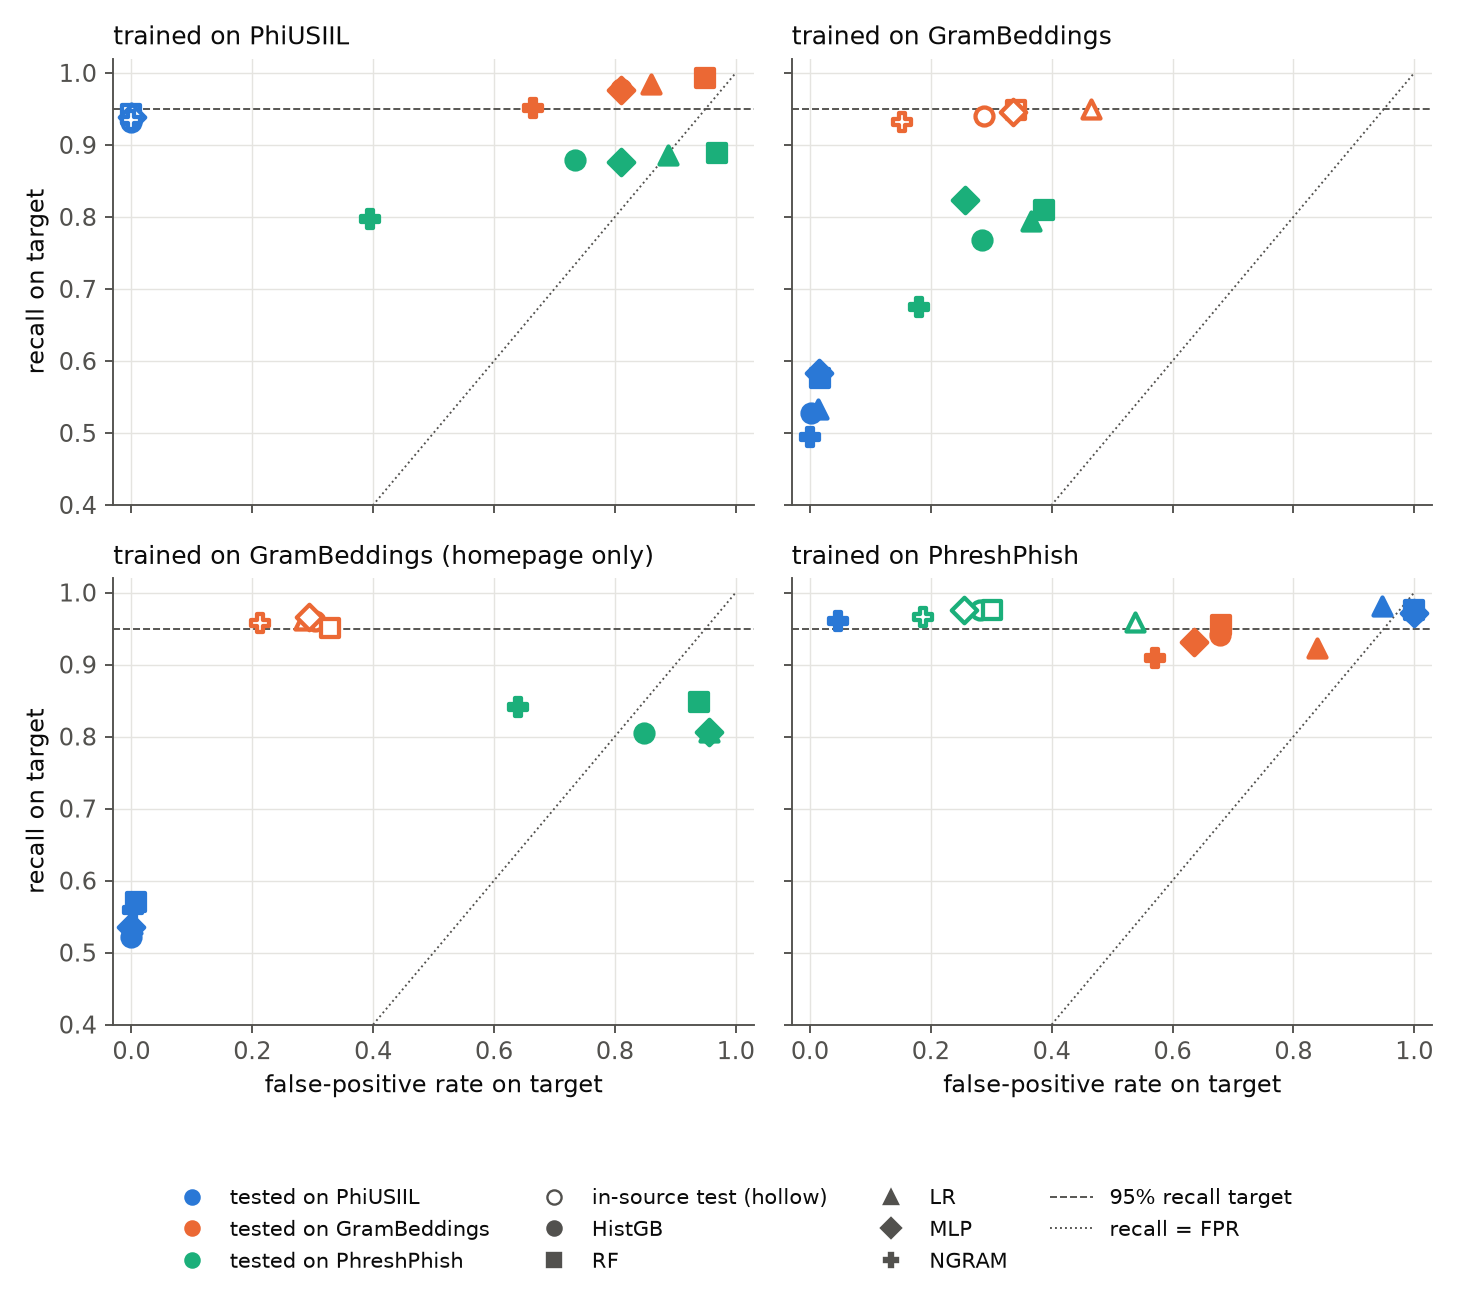
\includegraphics[width=0.88\textwidth]{fig_operating_points_2x2.png}
\caption{Recall and false-positive rate on each target at the threshold fixed on source validation. Hollow markers: the source's own test split. Marker shape: model. Means over five seeds.}
\label{fig:op}
\end{figure}

\textbf{URL type.} Training on homepage-only GramBeddings does not help: on PhreshPhish its AUROC is 0.46 and FPR 0.85 (Table~\ref{tab:slices} in the appendix). The homepage and deep slices of each target behave differently, so URL type matters, but controlling for it does not restore transfer.

\textbf{PhishTank.} The PhishTank snapshot has only phishing URLs, so recall is the only valid number there, and it is not a detection metric by itself: recall on PhishTank is 0.84--0.96 for HistGB (Table~\ref{tab:phishtank} in the appendix) while the same models have FPR up to 1.00 on other targets. A high PhishTank recall is compatible with a detector that flags almost everything.

\section{Why transfer fails: how the sources differ}\label{sec:why}
\textbf{The sources differ in form even within a URL type (Table~\ref{tab:profile}).} Among homepage URLs, legitimate URLs end with ``/'' in 0\% of rows in PhiUSIIL, 53\% in GramBeddings and 100\% in PhreshPhish; phishing homepages show the same spread (0.44, 0.99, 0.66, and 0.81 for PhishTank).

\textbf{A model can tell the source from the URL alone, within a class (Table~\ref{tab:discr}).} Within the legitimate class, PhiUSIIL is almost perfectly separable from the other sources (AUROC 0.99 against GramBeddings, 1.00 against PhreshPhish), even for homepages only and without scheme and \texttt{www}. Within the phishing class every pair is separable (0.85--0.93) except PhreshPhish against PhishTank (0.71), which is consistent with PhreshPhish drawing on PhishTank (4.3\% of its phishing URLs are in my PhishTank snapshot). So the sources differ beyond ``phishing versus legitimate''. Separability does not identify the feature responsible, and source also correlates with collection period (GramBeddings 2019--21, PhiUSIIL phishing 2022--23, PhreshPhish 2024--25) and hosting mix, which this measurement cannot separate from URL style.

\begin{table}[t]
\centering
\caption{Source discriminator: AUROC of predicting the source from URL-only features within one class (HistGB, equal numbers per source, registered-domain-disjoint split, mean of three seeds).}
\label{tab:discr}
{\footnotesize
\begin{tabular}{llrrr}
\toprule
\textbf{Class} & \textbf{Pair of sources} & \textbf{All features} & \textbf{No scheme, no www} & \textbf{Homepages only} \\
\midrule
legit & GramBeddings vs PhreshPhish & 0.864 & 0.804 & 0.872 \\
legit & PhiUSIIL vs GramBeddings & 0.993 & 0.988 & 0.961 \\
legit & PhiUSIIL vs PhreshPhish & 1.000 & 1.000 & 1.000 \\
phish & GramBeddings vs PhishTank & 0.904 & 0.867 & 0.856 \\
phish & GramBeddings vs PhreshPhish & 0.926 & 0.902 & 0.885 \\
phish & PhiUSIIL vs GramBeddings & 0.920 & 0.909 & 0.892 \\
phish & PhiUSIIL vs PhishTank & 0.864 & 0.847 & 0.862 \\
phish & PhiUSIIL vs PhreshPhish & 0.856 & 0.850 & 0.850 \\
phish & PhreshPhish vs PhishTank & 0.707 & 0.695 & 0.701 \\
\bottomrule
\end{tabular}
}

\end{table}

\textbf{Which features separate the sources (Table~\ref{tab:imp}).} I repeated the discriminator on homepage URLs and on deep URLs separately and measured permutation importance (the AUROC lost when one feature is shuffled on the held-out part). On homepages the importance sits in formatting: summed over all pairs and classes, \texttt{is\_https}, \texttt{has\_www} and \texttt{path\_len} carry 82\% of it, and on legitimate homepages \texttt{path\_len} is exactly the trailing slash (0 or 1, matching the slash in every row of all three sources). On deep URLs those three carry 32\%, and the rest falls on \texttt{entropy}, \texttt{path\_depth}, \texttt{url\_len}, \texttt{host\_len}, \texttt{n\_subdomains} and \texttt{digit\_ratio}, which describe the structure of the path and host. This fits the canonical-URL result below: normalizing removes the homepage formatting but not these structural differences. Caveats: permutation importance is split among correlated features and rests on three seeds, and a feature being important for separating sources does not by itself show that it causes a transfer failure.

\begin{table}[t]
\centering
\caption{Top two features (permutation importance) for telling the sources apart, within a class, on homepage URLs and on deep URLs. AUROC of the discriminator on that subset. n/a: PhiUSIIL has no deep legitimate URLs.}
\label{tab:imp}
{\footnotesize\setlength{\tabcolsep}{4pt}
\begin{tabular}{llrlrl}
\toprule
\textbf{Class} & \textbf{Pair of sources} & \textbf{Homepage AUROC} & \textbf{Top features, homepages} & \textbf{Deep AUROC} & \textbf{Top features, deep URLs} \\
\midrule
legit & GramBeddings vs PhreshPhish & 0.87 & path\_len, is\_https & 0.87 & is\_https, path\_len \\
legit & PhiUSIIL vs GramBeddings & 0.96 & has\_www, is\_https & n/a & n/a \\
legit & PhiUSIIL vs PhreshPhish & 1.00 & path\_len, n\_dots & n/a & n/a \\
phish & GramBeddings vs PhishTank & 0.86 & is\_https, path\_len & 0.94 & is\_https, n\_subdomains \\
phish & GramBeddings vs PhreshPhish & 0.89 & path\_len, is\_https & 0.92 & path\_depth, is\_https \\
phish & PhiUSIIL vs GramBeddings & 0.89 & path\_len, is\_https & 0.85 & entropy, path\_depth \\
phish & PhiUSIIL vs PhishTank & 0.86 & has\_www, is\_https & 0.86 & url\_len, entropy \\
phish & PhiUSIIL vs PhreshPhish & 0.85 & is\_https, has\_www & 0.82 & entropy, path\_len \\
phish & PhreshPhish vs PhishTank & 0.70 & path\_len, is\_https & 0.60 & path\_len, host\_len \\
\bottomrule
\end{tabular}
}

\end{table}

\textbf{Normalizing URL form does not repair transfer (Table~\ref{tab:canon}, Figure~\ref{fig:canon}).} I recompute the features on a canonical URL (lowercase, no scheme, no leading \texttt{www.}, no trailing ``/'') and, for the n-gram model, read the canonical string. In-source AUROC falls (for example, PhiUSIIL-trained HistGB from 0.997 to 0.847), so part of the in-source separability was formatting. But mean cross-source AUROC falls for four of the five models and is about equal for random forest, and the cross-source FPR at the fixed threshold rises (HistGB 0.55 to 0.74). What remains after normalizing, host and path content, brand and hosting mix, is not removed by cleaning URLs. The canonical form also drops genuine signal (https, \texttt{www}), so it is not a pure formatting control.

\begin{table}[t]
\centering
\caption{Cross-source and in-source AUROC for raw URLs, URLs without scheme and \texttt{www}, and canonical URLs. Mean over five seeds and over the eight source--target pairs (cross-source) or four sources (in-source).}
\label{tab:canon}
{\scriptsize\setlength{\tabcolsep}{3.5pt}
\begin{tabular}{lrrrrrr}
\toprule
\textbf{Model} & \textbf{Cross: raw} & \textbf{Cross: no scheme/www} & \textbf{Cross: canonical} & \textbf{In-source: raw} & \textbf{In-source: no scheme/www} & \textbf{In-source: canonical} \\
\midrule
HistGB & 0.694 & 0.651 & 0.667 & 0.965 & 0.957 & 0.908 \\
RF & 0.651 & 0.607 & 0.665 & 0.961 & 0.953 & 0.899 \\
LR & 0.693 & 0.593 & 0.618 & 0.949 & 0.916 & 0.889 \\
MLP & 0.683 & 0.623 & 0.662 & 0.965 & 0.935 & 0.912 \\
NGRAM & 0.819 & 0.754 & 0.757 & 0.977 & 0.948 & 0.942 \\
\bottomrule
\end{tabular}
}

\end{table}
\begin{figure}[t]
\centering
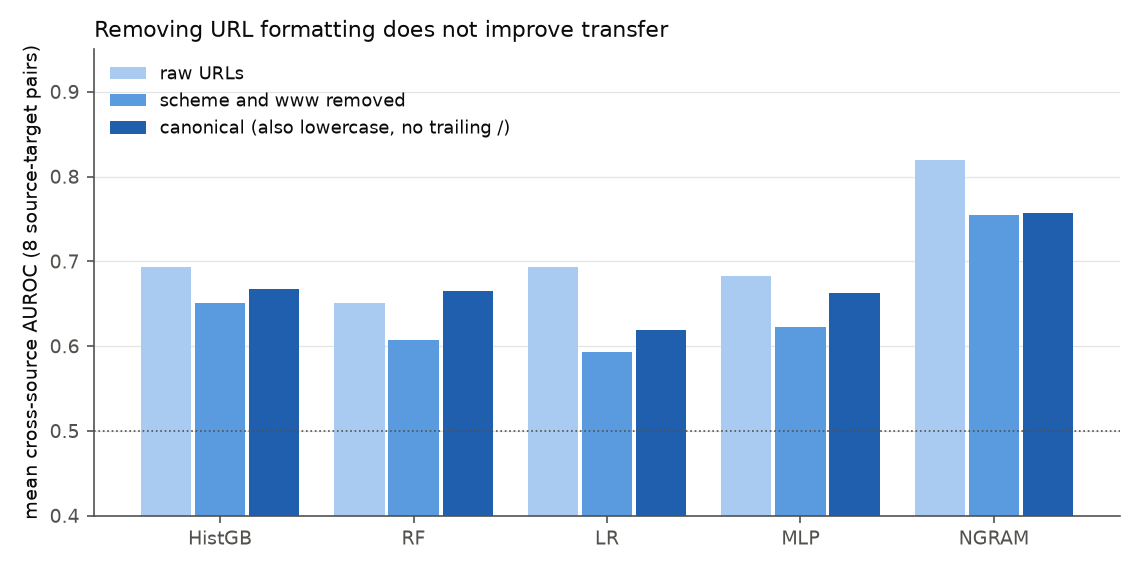
\includegraphics[width=0.62\textwidth]{fig_canonical_vs_raw.png}
\caption{Mean cross-source AUROC by model and URL form.}
\label{fig:canon}
\end{figure}

\textbf{Score distributions explain the opposite failure directions (Figure~\ref{fig:scores} in the appendix).} The PhiUSIIL-trained model puts nearly every URL from the other sources at a score near 1, legitimate and phishing alike, so the validation threshold flags them all. GramBeddings-trained models put PhiUSIIL legitimate URLs near 0 and also a large share of PhiUSIIL phishing (recall is 0.53 over five seeds for HistGB, 0.59 in the seed shown), so recall drops while FPR stays near 0.

\textbf{Provenance.} The GramBeddings documentation states a custom crawler and a manual filter for legitimate URLs but does not state the phishing source, the crawl seeds, whether legitimate URLs are homepages, or any preprocessing. I therefore cannot attribute the differences to a specific collection step.

\textbf{Why more data from the same sources is unlikely to resolve this.} The differences above look like properties of how each source was assembled, not of sample size: a source discriminator finds them within a class, they persist for homepages and without scheme and \texttt{www}, and canonical URLs do not remove them. A larger sample of a source would reproduce that source's form. I did not test this by scaling up (the full 800,000-row GramBeddings featurization was not run), so this is an argument from the measurements, not a measured result. What these differences call for is an independently assembled target, which the third source supplies, and a report of fixed-threshold FPR on each source.

\section{Limitations}
(1) Part B pools are small (11,666 rows per variant) because the homepage-only variant is small, and domain-disjoint splits are uneven because a few hosting domains (for example \texttt{gitbook.io}, \texttt{webflow.io}) hold 2--3\% of a pool each; in the seeds I checked, validation phishing share ranged from 0.35 to 0.57 across seeds and sources, so single-seed fixed-threshold numbers are noisy and I report five-seed means with standard deviations. (2) Removing domains seen in training also removes hosting-platform phishing, which is common in recent data; 55\% of PhreshPhish phishing rows share a registered domain with PhiUSIIL, mostly through such platforms. (3) Only 22 lexical features are used in Part B; page content, host and temporal features may transfer differently. (4) Source, collection period and hosting mix are confounded, and the GramBeddings and PhreshPhish provenance is incompletely documented. (5) GramBeddings and PhreshPhish are used as 100,000-row balanced samples, not in full. (6) PhishTank offers only recall. (7) The headline Part B table uses HistGB; the recall and FPR pattern agrees across five models, but pair-level AUROC does not. (8) The related-work numbers are quoted at the level I verified, mostly abstracts.

\section{Conclusion}
The paper's 99\% reproduces, but it is a property of this dataset's construction, not evidence that the detector finds phishing: the headline survives removing the similarity index and is reproducible from URL form alone. A URL-only detector trained on one of three sources does not carry its operating point to the others, in different directions for different pairs, and an oracle threshold would not repair most of them. The sources are separable within a class, and normalizing URL form does not fix transfer. For work on this benchmark I would report fixed-threshold recall \emph{and} false-positive rate on at least one independently collected source that has legitimate URLs of the same kind, check whether the source can be recovered within a class, and not rely on phishing-only recall.

\begin{thebibliography}{9}\small
\bibitem{prasad2024} A.~Prasad and S.~Chandra. PhiUSIIL: A diverse security profile empowered phishing URL detection framework based on similarity index and incremental learning. \emph{Computers \& Security}, 136, 2024. doi:10.1016/j.cose.2023.103545.
\bibitem{ahamed2026} T.~Ahamed, S.~C.~Kakon, F.~Al~Farid, J.~Uddin, and H.~B.~Abdul~Karim. An integrated evaluation protocol for adversarial robustness, generalization, and explanation stability in URL-based phishing detection. \emph{Frontiers in Computer Science}, 2026. doi:10.3389/fcomp.2026.1834407.
\bibitem{misiek2026} M.~Misiek and T.~Hyla. XGBoost-based URL phishing detection method with cross-dataset validation. \emph{IEEE Access}, 2026. doi:10.1109/ACCESS.2026.3672690.
\bibitem{rashid2024} F.~Rashid, B.~Doyle, S.~C.~Han, and S.~Seneviratne. Phishing URL detection generalisation using unsupervised domain adaptation. \emph{Computer Networks}, 245, 2024. doi:10.1016/j.comnet.2024.110398.
\bibitem{rahman2026} M.~H.~Rahman, Z.~Abidin, and M.~A.~Hariyadi. Enhancing phishing website detection using artificial neural network with logic gate-based feature interaction modeling. \emph{G-Tech: Jurnal Teknologi Terapan}, 10(3):1276--1289, 2026. doi:10.70609/g-tech.v10i3.10280.
\bibitem{arp2022} D.~Arp, E.~Quiring, F.~Pendlebury, A.~Warnecke, F.~Pierazzi, C.~Wressnegger, L.~Cavallaro, and K.~Rieck. Dos and don'ts of machine learning in computer security. In \emph{USENIX Security}, 2022.
\bibitem{dalton2025} T.~Dalton, H.~Gowda, G.~Rao, S.~Pargi, A.~Hadj~Khodabakhshi, J.~Rombs, S.~Jou, and M.~Marwah. PhreshPhish: A real-world, high-quality, large-scale phishing website dataset and benchmark. arXiv:2507.10854, 2025.
\bibitem{gram} A.~S.~Bozkir, F.~C.~Dalgic, and M.~Aydos. GramBeddings: A new neural network for URL based identification of phishing web pages through n-gram embeddings. \emph{Computers \& Security}, 124:102964, 2023. doi:10.1016/j.cose.2022.102964. Dataset: \url{https://web.cs.hacettepe.edu.tr/~selman/grambeddings-dataset/}; code: \url{https://github.com/fcdalgic/GramBeddings}.
\end{thebibliography}

\appendix
\section{Additional tables and figures}
\begin{table}[h]
\centering
\caption{Batch baselines (the paper's Table 3), held-out stratified 80/20 split, mean over five seeds. The paper does not state its split. HistGB stands in for LightGBM.}
\label{tab:t3}
{\footnotesize
\begin{tabular}{lrrr}
\toprule
\textbf{Model} & \textbf{Paper accuracy} & \textbf{Ours, 43 selected features} & \textbf{Ours, 21 URL-only features} \\
\midrule
BernoulliNB & 0.98644 & 0.98789 (0.00051) & 0.93714 (0.00109) \\
MultinomialNB & 0.68961 & 0.67323 (0.00226) & 0.77806 (0.00177) \\
PassiveAggressive & 0.98021 & 0.97728 (0.01478) & 0.99698 (0.00024) \\
Perceptron & 0.98041 & 0.97985 (0.01151) & 0.99513 (0.00261) \\
SGD & 0.94294 & 0.98365 (0.01268) & 0.99645 (0.00029) \\
LR & 0.99654 & 0.99992 (0.00003) & 0.99635 (0.00037) \\
DT & 0.99866 & 1.00000 (0.00000) & 0.99534 (0.00021) \\
RF & 0.99982 & 1.00000 (0.00001) & 0.99681 (0.00034) \\
AdaBoost & 0.99981 & 0.99998 (0.00003) & 0.98966 (0.00062) \\
GradientBoosting & 0.99978 & 1.00000 (0.00000) & 0.99561 (0.00046) \\
HistGB & 0.99990 & 1.00000 (0.00001) & 0.99740 (0.00037) \\
Bagging & 0.99923 & 1.00000 (0.00001) & 0.99652 (0.00027) \\
KNN & 0.99378 & 0.99888 (0.00012) & 0.99673 (0.00029) \\
MLP & not in paper & 0.99992 (0.00005) & 0.99806 (0.00023) \\
\bottomrule
\end{tabular}
}

\end{table}
\begin{table}[h]
\centering
\caption{HistGB on URL-type slices of each target. AUROC and FPR are undefined when the slice has only phishing URLs.}
\label{tab:slices}
{\footnotesize
\begin{tabular}{llrrrr}
\toprule
\textbf{Trained on} & \textbf{Tested on} & \textbf{n} & \textbf{AUROC} & \textbf{Recall} & \textbf{FPR} \\
\midrule
PhiUSIIL/all & GramBeddings homepage & 11{,}668 & 0.80$\pm$0.01 & 0.95$\pm$0.01 & 0.68$\pm$0.00 \\
PhiUSIIL/all & GramBeddings deep & 81{,}838 & 0.75$\pm$0.04 & 0.98$\pm$0.01 & 0.83$\pm$0.05 \\
PhiUSIIL/all & PhreshPhish homepage & 19{,}496 & 0.71$\pm$0.03 & 0.77$\pm$0.06 & 0.51$\pm$0.01 \\
PhiUSIIL/all & PhreshPhish deep & 63{,}503 & 0.76$\pm$0.03 & 0.97$\pm$0.01 & 0.75$\pm$0.14 \\
GramBeddings/all & PhiUSIIL homepage & 194{,}602 & 0.76$\pm$0.04 & 0.38$\pm$0.06 & 0.00$\pm$0.00 \\
GramBeddings/all & PhiUSIIL deep & 24{,}706 & n/a (one class) & 0.89$\pm$0.02 & n/a (phishing only) \\
GramBeddings/all & PhreshPhish homepage & 23{,}476 & 0.68$\pm$0.03 & 0.67$\pm$0.04 & 0.41$\pm$0.03 \\
GramBeddings/all & PhreshPhish deep & 68{,}605 & 0.86$\pm$0.00 & 0.85$\pm$0.02 & 0.27$\pm$0.03 \\
GramBeddings/homepage & PhiUSIIL homepage & 192{,}726 & 0.74$\pm$0.04 & 0.34$\pm$0.05 & 0.00$\pm$0.00 \\
GramBeddings/homepage & PhiUSIIL deep & 25{,}143 & n/a (one class) & 0.93$\pm$0.02 & n/a (phishing only) \\
GramBeddings/homepage & PhreshPhish homepage & 22{,}887 & 0.61$\pm$0.03 & 0.64$\pm$0.05 & 0.46$\pm$0.06 \\
GramBeddings/homepage & PhreshPhish deep & 68{,}662 & 0.58$\pm$0.02 & 0.94$\pm$0.01 & 0.88$\pm$0.03 \\
PhreshPhish/all & PhiUSIIL homepage & 191{,}066 & 0.60$\pm$0.02 & 0.99$\pm$0.00 & 1.00$\pm$0.00 \\
PhreshPhish/all & PhiUSIIL deep & 21{,}942 & n/a (one class) & 0.91$\pm$0.04 & n/a (phishing only) \\
PhreshPhish/all & GramBeddings homepage & 12{,}587 & 0.47$\pm$0.05 & 0.99$\pm$0.01 & 0.94$\pm$0.03 \\
PhreshPhish/all & GramBeddings deep & 83{,}165 & 0.77$\pm$0.01 & 0.94$\pm$0.02 & 0.63$\pm$0.07 \\
\bottomrule
\end{tabular}
}

\end{table}
\begin{table}[h]
\centering
\caption{Recall on the PhishTank snapshot (phishing only) at the validation-fixed threshold, mean$\pm$sd over five seeds.}
\label{tab:phishtank}
{\footnotesize
\begin{tabular}{lrrrrr}
\toprule
\textbf{Trained on} & \textbf{HistGB} & \textbf{RF} & \textbf{LR} & \textbf{MLP} & \textbf{NGRAM} \\
\midrule
PhiUSIIL/all & 0.95$\pm$0.00 & 0.97$\pm$0.00 & 0.95$\pm$0.00 & 0.94$\pm$0.03 & 0.73$\pm$0.06 \\
GramBeddings/all & 0.84$\pm$0.05 & 0.87$\pm$0.05 & 0.68$\pm$0.03 & 0.80$\pm$0.06 & 0.68$\pm$0.09 \\
GramBeddings/homepage & 0.84$\pm$0.03 & 0.94$\pm$0.01 & 0.93$\pm$0.01 & 0.92$\pm$0.03 & 0.80$\pm$0.05 \\
PhreshPhish/all & 0.96$\pm$0.02 & 0.95$\pm$0.03 & 0.97$\pm$0.04 & 0.95$\pm$0.03 & 0.95$\pm$0.02 \\
\bottomrule
\end{tabular}
}

\end{table}
\begin{table}[h]
\centering
\caption{HistGB AUROC and PR-AUC (mean$\pm$sd over five seeds) with the phishing share of each target. PR-AUC depends on that share.}
\label{tab:prauc}
{\footnotesize
\begin{tabular}{llrrr}
\toprule
\textbf{Trained on} & \textbf{Tested on} & \textbf{Phishing share} & \textbf{AUROC} & \textbf{PR-AUC} \\
\midrule
PhiUSIIL & in-source test & 0.46 & 1.00$\pm$0.00 & 1.00$\pm$0.00 \\
 & GramBeddings & 0.47 & 0.76$\pm$0.03 & 0.71$\pm$0.06 \\
 & PhreshPhish & 0.41 & 0.67$\pm$0.04 & 0.56$\pm$0.07 \\
\addlinespace
GramBeddings & in-source test & 0.48 & 0.94$\pm$0.01 & 0.95$\pm$0.01 \\
 & PhiUSIIL & 0.39 & 0.83$\pm$0.02 & 0.84$\pm$0.03 \\
 & PhreshPhish & 0.47 & 0.80$\pm$0.01 & 0.78$\pm$0.02 \\
\addlinespace
GramBeddings (homepage only) & in-source test & 0.54 & 0.95$\pm$0.02 & 0.95$\pm$0.04 \\
 & PhiUSIIL & 0.38 & 0.82$\pm$0.02 & 0.84$\pm$0.02 \\
 & PhreshPhish & 0.46 & 0.46$\pm$0.01 & 0.51$\pm$0.02 \\
\addlinespace
PhreshPhish & in-source test & 0.55 & 0.97$\pm$0.01 & 0.98$\pm$0.01 \\
 & PhiUSIIL & 0.37 & 0.49$\pm$0.02 & 0.56$\pm$0.04 \\
 & GramBeddings & 0.48 & 0.73$\pm$0.02 & 0.67$\pm$0.03 \\
\bottomrule
\end{tabular}
}

\end{table}
\begin{table}[h]
\centering
\caption{Class and URL-type mix of the sets used in Part B (seed 0). Targets are after removing URLs and domains seen in training.}
\label{tab:mix}
{\footnotesize\setlength{\tabcolsep}{4pt}
\begin{tabular}{llrrrr}
\toprule
\textbf{Trained on} & \textbf{Set} & \textbf{Rows} & \textbf{Phishing share} & \textbf{Homepage share, phishing} & \textbf{Homepage share, legitimate} \\
\midrule
PhiUSIIL/all & train & 8{,}407 & 0.51 & 0.73 & 1.00 \\
 & val & 1{,}487 & 0.40 & 0.66 & 1.00 \\
 & source test & 1{,}772 & 0.52 & 0.72 & 1.00 \\
 & GramBeddings all & 92{,}128 & 0.46 & 0.09 & 0.15 \\
 & PhreshPhish all & 78{,}380 & 0.37 & 0.43 & 0.07 \\
\addlinespace
GramBeddings/all & train & 8{,}352 & 0.52 & 0.11 & 0.15 \\
 & val & 1{,}742 & 0.44 & 0.11 & 0.13 \\
 & source test & 1{,}572 & 0.46 & 0.13 & 0.16 \\
 & PhiUSIIL all & 228{,}354 & 0.41 & 0.73 & 1.00 \\
 & PhreshPhish all & 94{,}152 & 0.48 & 0.46 & 0.07 \\
\addlinespace
GramBeddings/homepage & train & 7{,}909 & 0.48 & 1.00 & 1.00 \\
 & val & 1{,}447 & 0.38 & 1.00 & 1.00 \\
 & source test & 2{,}310 & 0.63 & 1.00 & 1.00 \\
 & PhiUSIIL all & 214{,}504 & 0.37 & 0.69 & 1.00 \\
 & PhreshPhish all & 91{,}798 & 0.47 & 0.47 & 0.07 \\
\addlinespace
PhreshPhish/all & train & 7{,}907 & 0.51 & 0.38 & 0.08 \\
 & val & 1{,}638 & 0.35 & 0.42 & 0.06 \\
 & source test & 2{,}121 & 0.58 & 0.69 & 0.08 \\
 & PhiUSIIL all & 208{,}515 & 0.36 & 0.72 & 1.00 \\
 & GramBeddings all & 94{,}172 & 0.48 & 0.11 & 0.15 \\
\bottomrule
\end{tabular}
}

\end{table}
\begin{figure}[h]
\centering
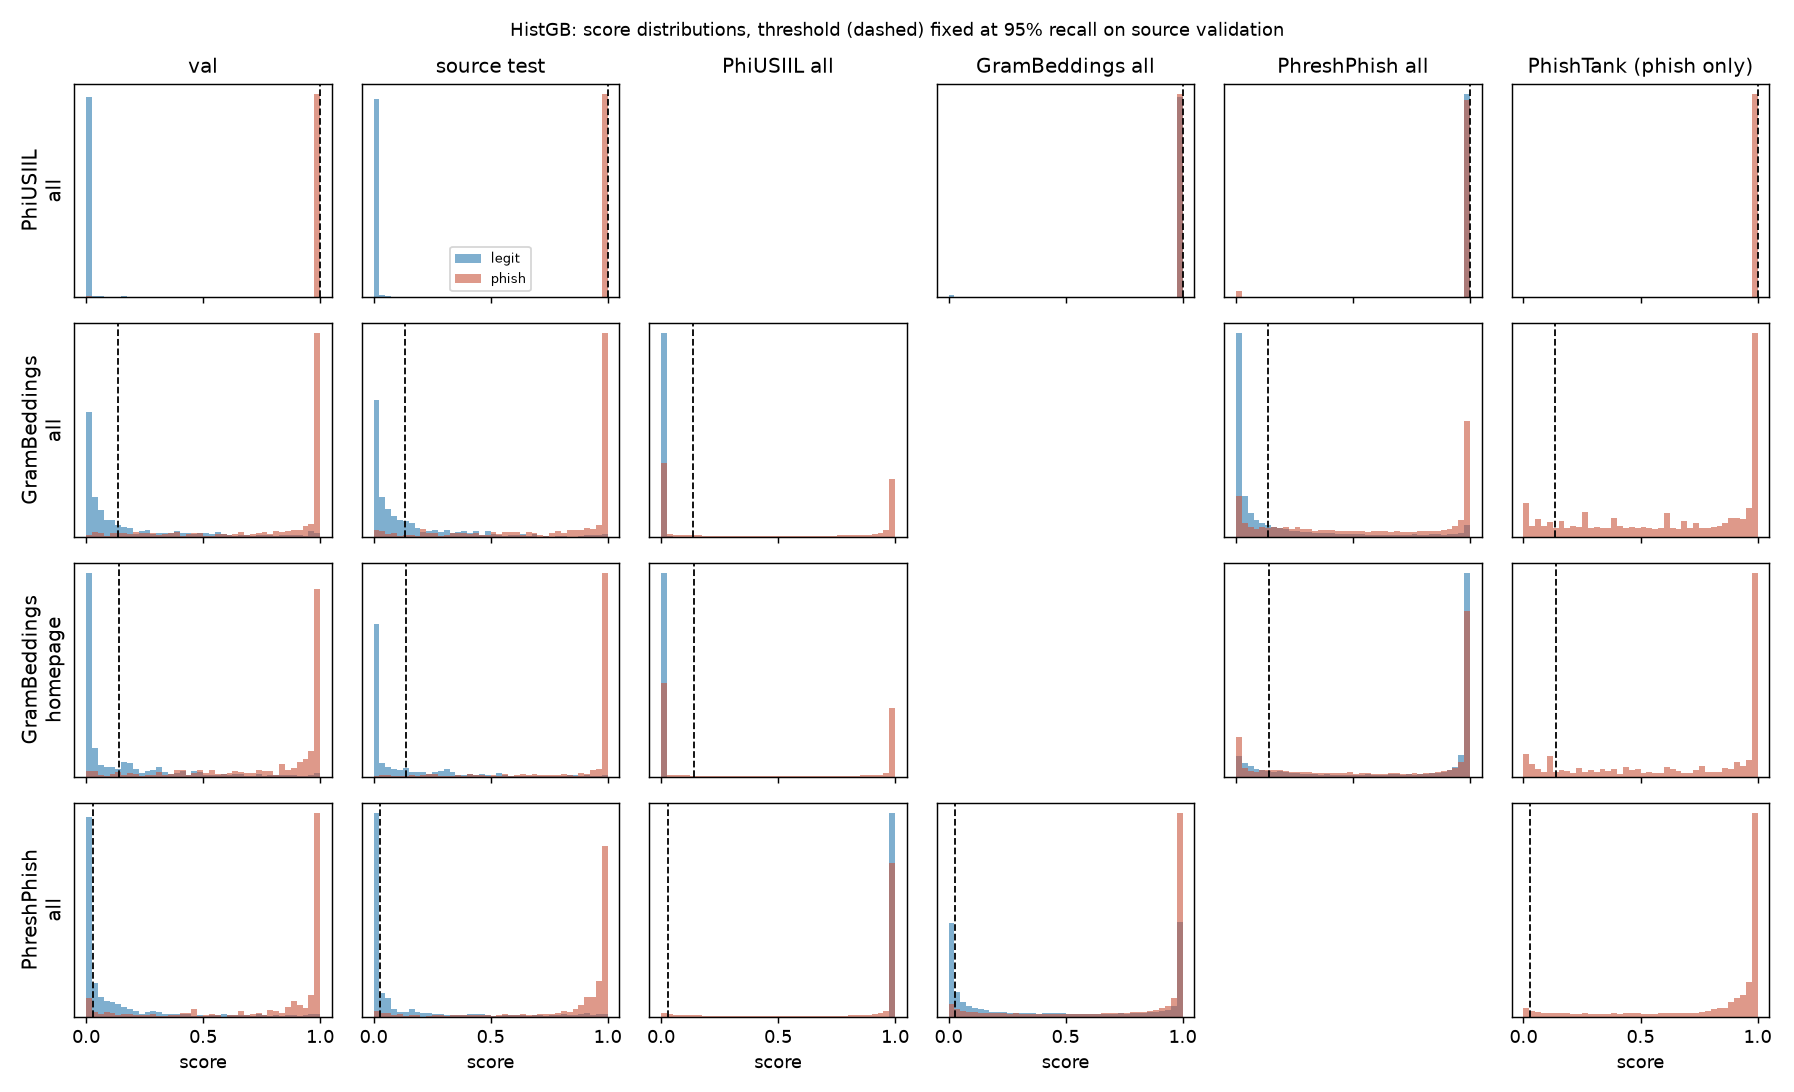
\includegraphics[width=\textwidth]{fig_scores_HistGB.png}
\caption{HistGB score distributions, seed 0: rows are training sources, columns are source validation, source test and each target. Dashed line: threshold fixed at 95\% recall on source validation.}
\label{fig:scores}
\end{figure}

\section{Hardware, timing and reproducibility}
All experiments ran on one laptop (Apple M4, 10 cores, 24 GB RAM, CPU only) with Python 3.14 and the package versions in \texttt{requirements.txt}. The incremental reproduction takes about 3 minutes per run for Tables 5 and 6 and about 20 minutes per mode for Table 7; the batch baselines take about 3 minutes in total; the five-seed transfer run (four sources, five models, three feature sets) took about 13.5 minutes, and the canonical-URL run about 4.6 minutes. Code, logs and result files are in \url{https://github.com/SuyashMuley/phiusiil-phishing-replication}. Final tables are generated by \texttt{scripts/16\_final\_tables\_figures.py}, \texttt{17\_final\_table\_partA.py} and \texttt{18\_make\_latex\_tables.py}.

\end{document}
